\documentclass{article}

\usepackage{amsmath, amsfonts, microtype, xcolor, tikz, graphicx, hyperref, amsthm}
\usepackage[ruled, linesnumbered]{algorithm2e}
\usepackage[]{neurips_2019}
\newtheorem{theorem}{Theorem}


\title{Measuring causal influence with\\ back-to-back regression: the linear case - supplementary material}

\begin{document}

\maketitle

\begin{figure}[h]
  \centering
  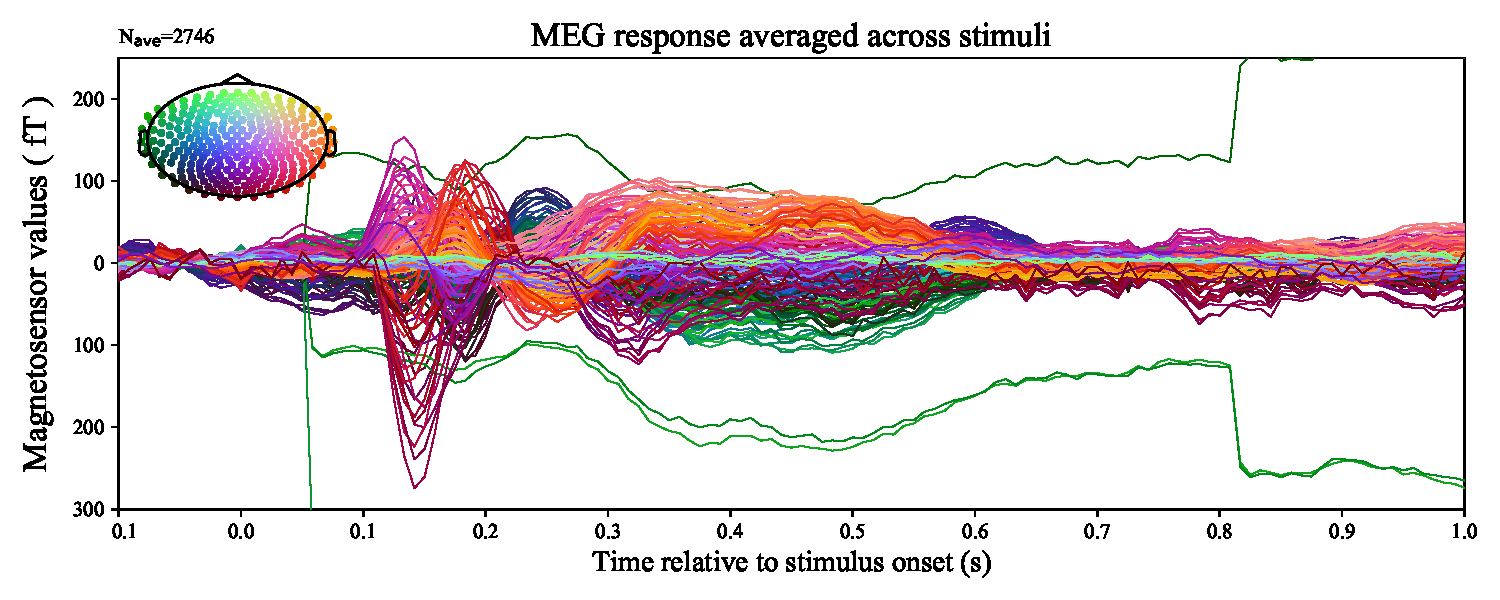
\includegraphics[width=\textwidth, trim=0cm 0cm 0cm 0cm, clip=True]{figures/meg_sensors.pdf}
  \caption{Magnetosensor response (femtoteslas fT) averaged across words for the first subject. The color coding corresponds to the positions of the sensors on the head as shown on the top-left diagram. The diverging curves correspond to artifacts in the MEG data.}
  \label{fig:megavg}
\end{figure}


\begin{figure}[h]
  \centering
  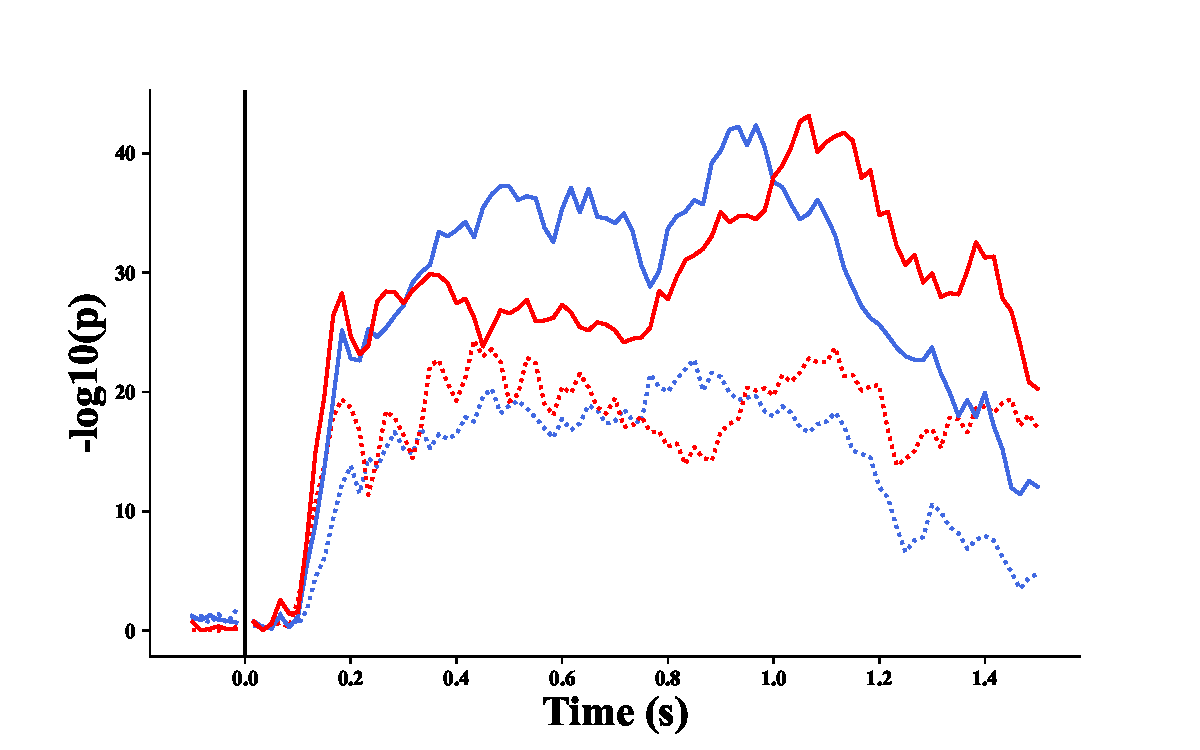
\includegraphics[width=\textwidth, trim=0cm 0cm 0cm 0cm]{figures/pvalues.pdf}
  \caption{We apply a statistical t-test to measure if coefficients were significantly different from baseline value (at word onset, $t=0$ms).
  We compute the negative logarithm of the p-value (\textit{higher is better}: nonzero effects are more easily detected). We plot the average across features, over time. Red: word length, blue: word frequency.
  Full line: B2B, dashed line: Forward regression. We see that our method more easily detects the influence of causes of MEG response.}
\end{figure}


\begin{figure}[h]
  \centering
  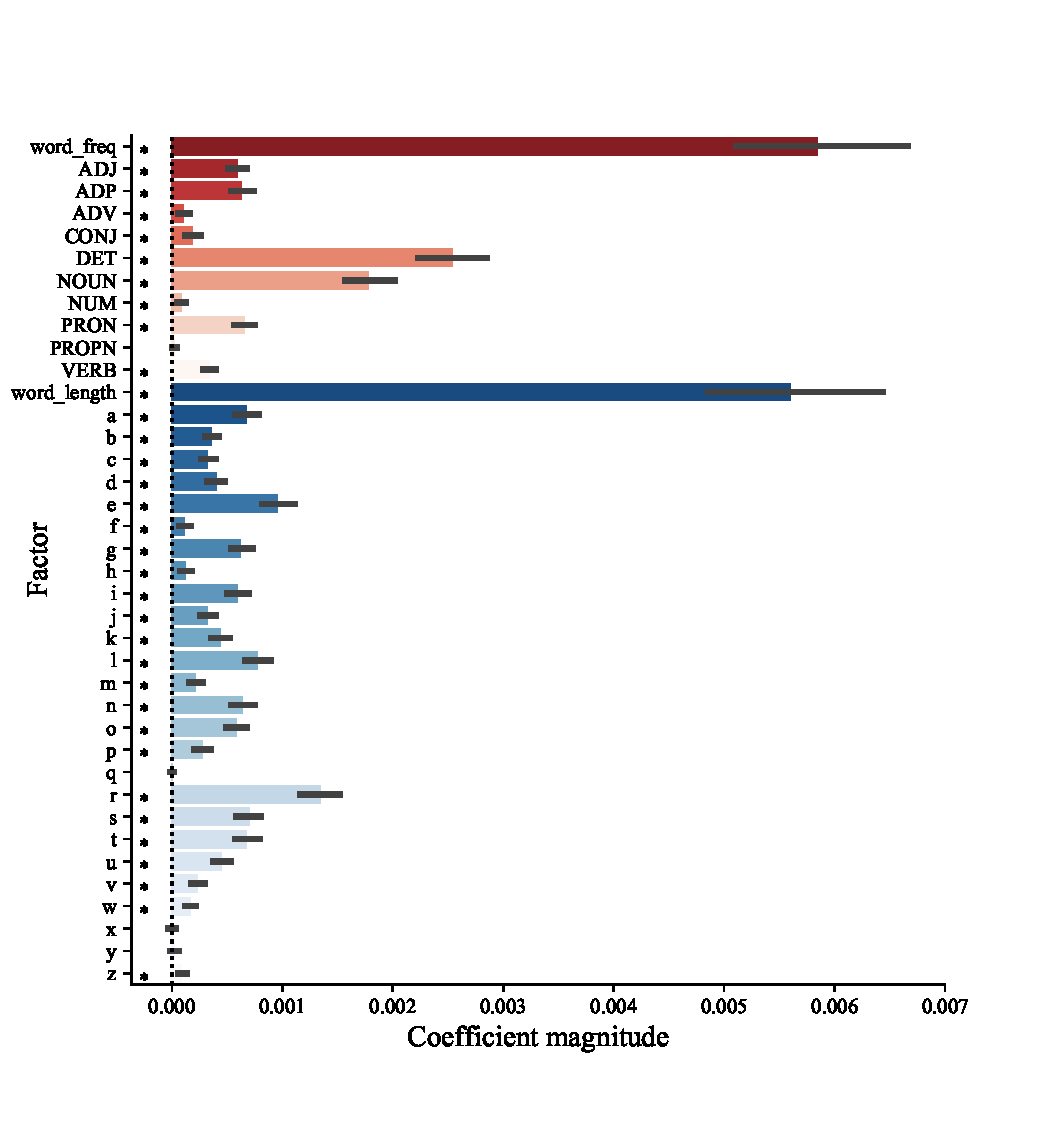
\includegraphics[width=\textwidth, trim=0cm 0cm 0cm 0cm]{figures/pvalues_vertical.pdf}
  \caption{We show the average value and the standard deviation across subjects of the coefficients obtained with our method during the trials. the $\star$  symbol corresponds to statistically significant (t-test) nonzero values.}
  \label{fig:ridgebaselineresult}
\end{figure}

\end{document}
